\documentclass{article}

\title{General Physics Study Guide}
\author{Ziyad Rahman \\ Email \href{zrahman3004@gmail.com}{zrahman3004@gmail.com} }
\date{}

\usepackage{hyperref}
\usepackage{amssymb}
\usepackage[english]{babel}
\usepackage{amsthm}
\usepackage{siunitx}
\usepackage{graphicx}
\graphicspath{{./images/}}

\begin{document}
\maketitle
\tableofcontents

\newpage
\section{Introduction}
This study guide is for General Physics I \& II. It covers basically all of the material in these courses. I can't guarantee it is all correct, but
I think it's fairly comprehensive. I took that course during \textbf{Fall 2024 \& Spring 2025} semesters, so that's when it was last updated. Material
could have changed or been moved around since then. Also, just to flag, the material is not in the order that it was taught the year I took it. I
grouped it based on concepts, rather than whatever the class does which I think is difficultly. As a result, you might encounter a really difficult
topic out of nowhere. For example, Forces and Torques are similar concepts, but Forces is the second chapter and Torques is one of the last in the class.
Despite that, I've decided to group them simply \textit{because} they are similar topics. With that out of the way, I hope you find this guide helpful!

\section{Prerequisite Math}

Obviously physics needs a lot of math. This section covers is mostly about vector math you'll need for this course.

\subsection{Special Angles}

Here are very common angles that may be asked of you. It's best to memorize these angles and their
values when trigonometric functions are used on them. These angles are reference angles, and because
of that, they only represent magnitude. You need to add the sign after you are done computing the value based
on what is physically happening in the scenario/question.

\begin{center}
\begin{tabular}{| c | c | c | c | c | c |}
    \hline
    Operation & $\ang{0} = 0 $ & $\ang{30} = \frac{\pi}{6}$ & $\ang{45} = \frac{\pi}{4}$ & $\ang{60} = \frac{\pi}{3}$ & $\ang{90} = \pi$ \\
    \hline
    $\sin (\theta)$ & 0 & $\frac{1}2$ & $\frac{\sqrt{2}}{2}$ & $\frac{\sqrt{3}}{2}$ & $1$ \\
    \hline
    $\cos (\theta)$ & 1 & $\frac{\sqrt{3}}{2}$ & $\frac{\sqrt{2}}{2}$ & $\frac{1}2$ & $0$ \\
    \hline
    $\tan (\theta)$ & 0 & $\frac{1}{\sqrt{3}}$ & $1$ & $\sqrt{3}$ & undefined \\
    \hline
\end{tabular}
\end{center}

\subsection{Basic Vector Operation}
A vector is a way to store numbers. In a physics sense, it's really just an arrow pointing from one place to another. Below are vector basics
including how to add and multiply vectors. This covers all important vector operations done in this course. A normal number like \( 5 \) is
called a scalar. In this class if something is not a vector, then it is a scalr.

\subsubsection{Representing Vectors and Magnitude}
Let $\vec{A}$ be a vector of 3 dimensions.
\begin{equation}
    \vec{A} =  A_x \hat{i} + A_y \hat{j} + A_z \hat{k}
\end{equation}
There are other ways to represent vectors, but this is the way we'll do it in this class. Each \(A_{something}\) literally just represents the
$x$, $y$, or $z$ coordinate of the arrow's tip.

A quick notational thing is the difference between \( \vec{|A|} \) and \( \vec{A} \). The first one represents the magnitude while the second one
is the actual vector. If you think about our arrow representation, the magnitude of a vector is literally just how long it is. In a 2D space,
if you think about a triangle, think about it as finding the hypotenuse from the length of the base and height. In fact, to find the magnitude
of a vector from its normal form, you just use pythagorean's theorem. Below is that theorem in three dimensions.
\begin{equation}
    |\vec{A}| = \sqrt{A_x^2 + A_y^2 + A_z^2} 
\end{equation}

\subsubsection{Vector Addition and Subtraction}
\begin{equation}
    \vec{A} \pm \vec{B} = \langle \vec{A}_x \pm \vec{B}_x, \; \vec{A}_y \pm \vec{B}_y, \; \vec{A}_z \pm \vec{B}_z \rangle = \vec{C}
\end{equation}

\subsubsection{Vector Multiplication}
Vector multiplication comes in three flavors: multiplication by a scalar, the dot product, and the cross product. Scalar multiplication is multiplication
between a scalar and a vector. The other two occur between two vectors. On a super high level, the dot product results in a scalar, whereas the 
cross product creates another vector.

\noindent \textbf{Scalar Multiplication.} Multiplying a vector by a scalar is by far the easiest vector multiplication. Suppose $n$ is a scalar (that
is, $n$ is some number).
\begin{equation}
    n\vec{A} = (A_x \times n) \hat{i} + (A_y \times n) \hat{j} + (A_z \times n) \hat{k}
\end{equation}
You basically just distribute it over the vector.

\noindent \textbf{The Dot Product.}
There are two ways to calculate the dot product.
\begin{equation}
    \vec{A} \cdot \vec{B} = (\vec{A_x} \times \vec{B_x}) + (\vec{A_y} \times \vec{B_y}) + (\vec{A_z} \times \vec{B_z})
\end{equation}
\begin{equation}
    \vec{A} \cdot \vec{B} = |\vec{A}| \times |\vec{B}|\cos{\theta}
\end{equation}

This is the second equation solved for theta, which often comes in handy.
\begin{equation}
    \theta = \cos^{-1} \left( {\frac{\vec{A} \cdot \vec{B}}{|\vec{A}| \times |\vec{B}|}} \right)
\end{equation}

\noindent \textbf{The Cross Product.}
There are also two ways to calculate the cross product. A quick note: when you do the cross product of two 3D vectors, your resultant vector (the
output) will be one dimensions smaller. 

\begin{equation}
    \vec{A} \times \vec{B} = |\vec{A}||\vec{B}| \sin \theta
\end{equation}

\begin{equation}
    \vec{A} \times \vec{B} = (A_y \times B_z - A_z \times B_y)\hat{i} + (A_z \times B_x - A_x \times B_z)\hat{j} + (A_x \times B_y - A_y \times B_x)\hat{k} \\
\end{equation}
This formula will be used a lot less. In fact, you'll almost never use it.    

\section{Kinematics}
Kinematics refers to the process of figuring out how something moves over time, including its velocity and acceleration.

\subsection{Primer: Translational and Rotational Motion}
Before discussing how to actually do kinematics, we'll start by talking about the two types of motion studied in this class: translational and rotational.
\textbf{Translational} motion refers to things moving in a line or curve. For example, a car driving down the highway or a ball being thrown between two 
people. \textbf{Rotational} motion refers to the motion of something spinning such as someone on a merry go round or a pulley. 

Something can have one and not the other, both, or neither. If I have a bowling ball in my hand and I'm just holding it, then it is stationary, so
it has no motion. If I begin to spin the bowling ball on the floor and it stays in place, then it has rotational but not translational motion. If I
slide it (that is, it's not rolling, the holes are always at the top for instance) then it has translational but not rotational motion. If I throw it
down the alley and its rolling as it barrels towards the bowling pins, then it has both types of motion.

\subsection{Primary Kinematic Equations}
We start with $\vec{r}$ which represents position in a unit of distance (\textit{m}). Before we begin, this variable is a little weird. In most of the
equations given, you won't see a $\vec{r}$ because things will be generalized in one dimension. Just understand that $\vec{r} = x \; \hat{i} + 
y \; \hat{j} + z \; \hat{k}$.

We can think about our kinematic equations in very general terms using derivatives. The core kinematic equations are as follow.
\begin{equation}
    \vec{v} = \frac{\mathrm{d}\vec{r}}{\mathrm{d}t}
\end{equation}
\begin{equation}
    \vec{a} = \frac{\mathrm{d}\vec{v}}{\mathrm{d}t}
    \end{equation}

\subsubsection{Special Case: Constant Acceleration} \label{kinematics const a}
Then, we have the constant acceleration equations which is what you'll use more often.
    \begin{equation}\label{eq: kinematic 1}
    \vec{v}_f = \vec{v}_i + \vec{a}t
\end{equation}
\begin{equation}\label{eq: kinematic 2}
    \vec{r}_f = \vec{r}_i + \vec{v}_it+ \frac{1}{2}\vec{a}t^2 
\end{equation}
\begin{equation}\label{eq: kinematic 3}
    \vec{v}_f^{ \: 2} = \vec{v}_i^{ \: 2} + 2 \vec{a} (\vec{r}_f - \vec{r}_i)
\end{equation}
\subsubsection{Relative Kinematics Based on Postion}
Since positions are relative, we can deduce the relative speed of an object \textit{A} relative to a Point \textit{B} if we know the speed of \textit{A} 
relative to a position \textit{C} and the speed of \textit{C} relative to \textit{B}'s position. This applies to position, velocity, and acceleration. 
To solve for this, we can use the following formula.
\begin{equation}
    v_{\frac{A}{B}} = v_{\frac{A}{C}} +  v_{\frac{C}{B}}
\end{equation}

\subsection{Rotational Kinematics}
Just a quick note before this section begins. Appendix \ref{Appendix B} contains a useful chart that summarizes all of the translation and rotational 
counterparts. The section below provides a slightly more in-depth look at the topic, including useful formulas, but if you're just trying to remember 
what the rotational counterpart to displacement is, you might be better off checking the chart.

\subsubsection{Introducing Rotational Kinematics} \label{trans to ang}
Rotational kinematics operate in practically the same way as translational kinematics, but deals with objects that are spinning or otherwise 
moving in a circular motion.
Below, we detail how you can take tangential measurements and turn them into their rotational counterparts. \\
\[ \vec{s} = r \theta \]
\[ \vec{v} = r \omega \]
\[ \vec{a} = r \alpha \]
\[ t = t \]

In these equations, $\vec{r} = \vec{s}$ for clarity's sake because the $r$ that is included actually refers to the path's radius. Both $\vec{r}$ and 
$\vec{s}$ mean position. You would refer to each counterpart as the "angular" version of the translational one 
(ex. displacement becomes angular displacement).

\subsubsection{Primary Rotational Kinematics Equations}
Since we have already defined $\theta$ as angular displacement (in radians) we can define the other kinematic values.
\begin{equation}
    \omega = \frac{\mathrm{d}\theta}{\mathrm{d}t}
\end{equation}
\begin{equation}
    \alpha = \frac{\mathrm{d}\omega}{\mathrm{d}t}
\end{equation}

\subsubsection{Special Case: Constant Rotational Acceleration}
Now, we can combine the special case kinematic equations found in \ref{kinematics const a} with the definitions that relate the translational and angular values in \ref{trans to ang}. The process is simple, since the angular form of a kinematic value is the just the translational counterpart divided by $r$, we can just divide each of the \ref{kinematics const a} equations by $r$ to create rotational counterparts.
\begin{equation}
    \omega_f = \omega_i + \alpha t
\end{equation}
\begin{equation}
    \theta_f = \theta_i + \omega_it+ \frac{1}{2}\alpha t^2 
\end{equation}
\begin{equation}
    \omega_f^{ \: 2} = \omega_i^{ \: 2} + 2 \alpha  (\theta_f - \theta_i)
\end{equation}

\subsubsection{Period and Frequency}
As an object rotates around itself (or travels in a circular path), it's bound to come back to the same point eventually. Note that this only works for 
zero acceleration otherwise the time to finish one rotation would keep changing and that defeats the purpose of calculating such a measurement in the 
first place.The time it takes for one full rotation (usually called a cycle) is called the \textit{period}, recorded in some unit of time. 
\begin{equation}
    T = \frac{2 \pi}{\omega}
\end{equation}
\noindent \textit{Frequency} is the inverse of the period, defined as the number of rotations an object makes in one unit of time. Below are 
definitions of both in relation to angular velocity and each other.
\begin{equation}
    f = \frac{1}{T}
\end{equation}
An important thing to note is the unit of frequency. Since it's the inverse of $T$, its units are technically just "cycle per unit time", but if the 
unit of time is seconds, then we the unit hertz (\textit{hz}). In other words $hz = \frac{1}{s}$.

\subsubsection{Centripedal Acceleration}
Centripetal acceleration, or rotational acceleration, is another important value that is unique to rotational motion. In effect, it is the inward 
acceleration that keeps an object that is moving in a circular path in that path. For example, you might be swinging a ball on a string in a circle; 
the reason it doesn't fly out is because the sting is applying a force (and therefore accelerating the ball) back into the circle as tangential 
velocity "tries to get it" to fly out. We can define centripetal acceleration using both tangential velocity and angular velocity.
\begin{equation}
    \vec{a}_c = \frac{\vec{v}^{\: 2}}{r} = \omega^2 r
\end{equation}


\section{Forces}
\subsection{Reference Frames}
Reference frames, especially inertial reference frames, are an extremely important concept in the General Physics course. For the most part, homework 
and exam problems will exist within inertial reference frames, but it is still important to understand what a reference frame is and they relate to 
Newton's laws. \\

\noindent This subsection will discuss in the broadest terms what reference frames are. There is a lot more nuanced especially as you move into special 
relatively, but for the purposes of this study guide, I have boiled the concept down to the basic version we need to understand for this course.

\noindent \textbf{Reference Frame:} Refers to the parameters of observation, such as how the axes are situated or when $t=0$.

\noindent \textbf{Inertial Reference Frame:} Refers to a reference frame in which Newton's laws hold true. That is, we can identify every force 
acting on an object and determine that motion is consistent with Newton's three laws. If you find yourself in a non-inertial reference frame, you 
may do one of two things.
\begin{enumerate}
    \item Accept that you are in a non-inertial reference frame and calculate motion without Newton's laws.
    \item Accept that you are in a non-inertial reference frame, but add a "fake" or "non-existent" force which allows you to use Newton's laws.
\end{enumerate}
\textit{Example:} Say a person is in a car that moves along a curved road. There are two possible observation points, otherwise known as reference frames. The first is an outside observer standing at the side of the road, and the second frame is of the person sitting inside of the car.
\begin{enumerate}
    \item The observer on the side of the road \textit{is} in an inertial reference frame: \\
    From the observer's point of view, all motion can be explained using Newton's laws. Put simply, the observer can determine that the car is moving, that it is being pulled into the curve by centripetal acceleration (friction on the tires).
    \item The person inside the car \textit{is not} in an inertial reference frame: \\
    The person inside the car has a different perspective. From their reference frame, the road is moving, not them. Due to this, they cannot determine that they have a tangential velocity to the curve of the road, and therefore, they cannot explain why they are being pushed off the road.
    \begin{enumerate}
        \item They can either accept they are in a non-inertial reference frame and make calculations accordingly (without Newton's laws), or
        \item Accept they are in a non-inertial reference frame, but add a "fake" force pushing them outside the circle so that Newton's second law holds true. This allows them to use all of Newton's laws.
    \end{enumerate}
\end{enumerate}

\subsection{Newton's Laws}
\subsubsection{Newton's First Law: Inertia}
\textbf{Definition:} In an inertial frame of reference, if there is \textit{no} force on an object, then a stationary object remains at rest and '
an object in motion stays in motion with a constant velocity, $\vec{v}$.

\noindent \textbf{Sloadism Definition:} If there's no force on an object, then its movement doesn't change. If its stopped, it will stay stopped, if 
its moving, it'll keep moving at the same speed.

\subsubsection{Newton's Second Law: Force}
\textbf{Formal Definition:} In an inertial-reference frame, for an object of momentum $\vec{p}$, the net force is the change in momentum over time.

\noindent \textbf{Sloadism Definition:} The net force on an object is its impulse over time (or mass times acceleration).

\begin{equation}
    F_{net} = \frac{\mathrm{d}\vec{p}}{\mathrm{d}t} = m\vec{a}
\end{equation} 

\noindent{Where,} \\
$p = $ momentum of the object in newton-meters. \\
$t = $ time in seconds. \\
$m = $ the mass of the object in kilograms. \\
$a = $ the acceleration of the object in meters per second. \\

\subsubsection{Newton's Third Law: Action \& Reaction}
\textbf{Definition:} In an inertial reference frame, $F_{\mathrm{A \, on \, B}} = -F_{\mathrm{B \, on \, A}}$.

\noindent \textbf{Sloadism Definition:} Every action has an equal and opposite reaction.

Maybe add that thing about how the book and the table are not normal.

\subsection{Hooke's Law}
In physics, a lot of classic problems revolve around springs. Naturally, that means springs behave in a unique (but simple) way when it comes to
forces. We'll only be considering ideal springs. That is massless springs with a fixed stretchiness. Hooke's law is the equation we use to determine 
the amount of force it takes to stretch or compress a string (and by Newton's Third Law, how much force the spring is exerting on whatever its pushing
or pulling against). It is as follows:
\begin{equation}\label{eq : hooke}
    \vec{F}_{spring} = k \Delta s
\end{equation}

\noindent Where, \\
\indent $k$ is the elastic coefficient \\
\indent $\Delta s$ is the distance the spring has moved. You'll have to determine the direction just as you would any other force. You can think of
the direction of pointing towards the center (so if its stretched and you have a typical $x$ and $y$ axis, then the direction is the negative one).

\subsubsection{The Elastic Coefficient}
The elastic coefficient $k$ is a constant based on the spring/material that is being used. It describes how many newtons it takes to stretch or 
compress that material by one meter. It follows then that it's units are $\frac{N}{m}$.

\section{Torques}
Torques are the rotational equivalent to forces.
If forces cause translational acceleration, motivating an object to move translationally, then torque
motivates objects to move rotationally. Before we talk about torques, we'll first discuss the mass equivalent for rotational motion, then talk about
Newton's Rotational Laws and a few important scenarios.

To law a few ground rules, we represent torques with $\tau$ in $Nm$. The counter-clockwise direction is positive and the clockwise direction is negative.

\subsection{Moments of Inertia}
If mass is a measurement of how inert something is that means it measures how difficult something is to move (or otherwise to gain momentum). Likewise,
the \textbf{moment of inertia} measures how difficult it is to rotate something. More intuitively, it measures how far apart mass is spread from
something's pivot (the point it spins around). If two things have the same mass and one is packed closer, then it will have a smaller moment of inertia
compared to the second object who has the same mass spread across a larger distance (for example, if you have two balls with the same mass, the smaller
one has a smaller moment of inertia because the mass is spread out less). We represent the moment of inertia with the variable $I$ and its units are
$kgm^2$.

The moment of inertia depends on the shape of an object, so each one has a different formula (you use a different formula to calculate a disc's moment
of inertia than for a ball). These will always be given, so I won't bother detailing them here.

\subsubsection{The Parallel Axis Theorem}
This theorem is used to find the moment of inertia for an object who's pivot axis has moved but stayed parallel to itself. For example, if spin a ball
on my finger, then its axis is straight up (this would be $I_{original}$). If I instead decide to spin it by spinning in a circle with my arms out, then 
its axis is moved away from the center, but is still parallel (that is, straight up). To calculate the new moment of inertia, we can use the following
equation.
\begin{equation}
    I_{new} = I_{original} + md^2
\end{equation}
Where,
$m$ is the object's mass and \\
$d$ is the distance the axis moved.

\subsection{Newton's Rotational Laws}
Just like with forces, we have three laws to consider. We'll look at them out of order since the second one is more involved (and arguably important)
than the others. The same constraint that this must happen in an inertial reference frame applies.

\subsubsection{Newton's First Rotational Law}
In an inertial reference frame, if there is no torque acting on an object, then objects at rest stay at rest and objects in motion stay in motion with 
a constant velocity.

\subsubsection{Newton's Third Rotational Law}
In an inertial reference frame, torques are met with an equal and opposite reaction.
\begin{equation}
    \tau_{A on B} = - \tau_{B on A}
\end{equation}

\subsubsection{Newton's Second Rotational Law}
This is the same as Newton's Second Translation Law.
\begin{equation}
    \tau_{net} = I \alpha
\end{equation}

\section{Momentum}
Momentum is an extremely important concept that will come up time and time again in all types of ways. Very simply put, momentum looks at how inert
something is and how fast its moving. There are translational and angular (rotational) momentums. We'll start by discussing the properties of momentum 
with reference to translational momentum. Just know all of these qualities apply to angular momentum except for the one special case about angular
momentum. The momentum equation is as follows.
\begin{equation}
    \vec{p} = m \vec{v}.
\end{equation}
The unit is $\frac{Kgm}{s}$ or more simply $Ns$.

\subsection{Conservation of Momentum}
In all collisions for this class, momentum is conserved. That means 
\begin{equation}
    \vec{p}_{Initial} = \vec{p}_{Final}.
\end{equation}
This will be an extremely useful concept moving forward.

\subsection{Types of Collisions}
There are two types of collisions that may occur. \textbf{Elastic} and \textbf{Inelastic} collisions. 

\subsubsection{Elastic Collisions}
Elastic collisions (visually) occur when two objects hit and bounce off. That's a good rule of thumb and will apply to most cases in this course, but
we can also be more precise. An \textbf{Elastic Collision} is any collision that conserved momentum and kinetic energy (we'll talk about kinetic energy
in the next section. For now, just understand that its some property being conserved). In math terms,
\begin{eqnarray*}
    \vec{p}_{Initial} = \vec{p}_{Final} \\
    K_{Initial} = K_{Final}
\end{eqnarray*}

Since kinetic energy is conserved, we can actually write a special equation that makes it easier to solve for velocities. This only applies to
\textbf{1D collisions}.
\begin{equation}
    v_1 + v_1^\prime = v_2 + v_2^\prime
\end{equation}
The prime represents the final velocity for object one or object two. This \textbf{DOES NOT} apply to angular momentum since by definition it doesn't
happen in one dimension.

\subsubsection{Inelastic Collisions}
A good rule of thumb for this type of collision is when two things hit each other and stick together. In an \textbf{Inelastic Collision}, momentum is
conserved, but kinetic energy is not. So,
\begin{eqnarray*}
    \vec{p}_{Initial} = \vec{p}_{Final} \\
    K_{Initial} \neq K_{Final}
\end{eqnarray*}

\subsection{Impulse and Newton's Second Law Revisited}
The change in momentum is an important concept. We call the change in momentum "impulse" and represent it with a $J$.
\begin{equation}
    \vec{J} = \Delta \vec{p}.
\end{equation}

Earlier, we defined Newton's Second Law as
\begin{eqnarray*}
    F = \frac{\text{d} \vec{p}}{\text{d}t}
\end{eqnarray*}
Now you know what the $p$ means.

\subsection{Angular Momentum}
We'll conclude this section by talking about \textbf{angular momentum}, which is how inert and how fast something is rotationally. We write it
using the following equation.
\begin{equation}
    \vec{L} = I \omega = \vec{r} \times \vec{p}
\end{equation}
Notice how the second iteration involves the cross product. The ideas of two types of collisions and whatnot still apply. However, again note the special
equation for elastic equations doesn't.

We can also use angular momentum to define net torque.
\begin{equation}
    \tau_{net} = \frac{\text{d} \vec{L}}{\text{d} t}
\end{equation}

\subsubsection{Angular Momentum of an Object Moving Linearly}
We can actually determine the angular momentum of an object moving in a straight line. Consider the image below.

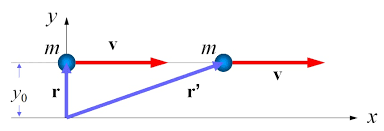
\includegraphics{linear_L.png}

First, we establish a "pivot" point. This is the point we are interested in the object's angular momentum around. We'll just have this be the
origin (where the two blue lines meet). To find the angular momentum in this case, we take the shortest distance between the path of the object
$r$. Then, just take the cross product with momentum (the second iteration of the angular momentum equation.)

\section{Work, Energy, and Power}
\subsection{Energy}
Energy, somewhat recursively, is the ability to do work (more on work
in a little bit). Energy is measured in \textit{joules} ($J$), which is equivalent to
$Nm$.

\subsubsection{Conservation of Energy}
Energy cannot be created or destroyed, only transferred. That means
that at some point A, the energy is equal to the energy at another
point B (if the system encompasses everything).

\begin{eqnarray} \nonumber
    E_A = E_B
\end{eqnarray}

\subsection{Work}
Work (joules) is the measure of energy transferred to an object when it is 
moved over a distance. The actual equation is as follows.

\begin{eqnarray} \label{eq : true work}
    \int \vec{F} \, \text{d}\vec{r}
\end{eqnarray}

\noindent Since this is technically not a calculus based course, we simplify
this equation in the following way.

\begin{eqnarray} \label{eq : work}
    W = \vec{F} \cdot \Delta \vec{r}
\end{eqnarray}

\noindent From this, we can draw a few conclusion that can simplify 
problem-solving. Expanded, we can rewrite the work formula as the
following.

\begin{eqnarray} \nonumber
    \vec{F} \cdot \Delta \vec{r} = F \Delta r \cos(\theta_{\vec{F} \Delta \vec{r}})
\end{eqnarray}

We can take the $\cos(\theta_{\vec{F} \Delta \vec{r}})$ term. From this we
can tell a few things. If the movement and the force are in the same
direction, then the work is positive. If they are in the opposite
direction, then work is negative. Last, if they are perpendicular,
the work is zero.

\subsection{Types of Energy}
There are several types of energy, but there are a few that are especially
important for this course. This section will go through each of these.

\subsubsection{Kinetic Energy}
Kinetic energy refers to the amount of energy in an object by
virtue of its motion.

\begin{equation}
    K = \frac{1}{2}mv^2 = \frac{p^2}{2m}
\end{equation}

We also have the rotational equivalent. This is the only energy type with a rotational equivalent.
\begin{equation}
    K_{Rotational} = \frac{1}{2} I \omega ^2
\end{equation}

\subsubsection{(Gravitational) Potential Energy}
Gravitational potential energy is the amount of stored energy in an
object relative to various parts of its system.

\begin{eqnarray}
    U_g = mg \Delta \vec{r}
\end{eqnarray}

\noindent Where, $\Delta \vec{r}$ is the displacement from an arbitrarily
chosen point. This will typically be a point that is chosen because it makes
calculations easier.

\subsubsection{Elastic (Potential) Energy}
The amount of energy stored in a spring.

\begin{eqnarray}
    U_s = \frac{1}{2} k \Delta \vec{x} \, ^2
\end{eqnarray}
Where, $\Delta \vec{x} \, ^2$ is the displacement of the spring
compared to where it in its equilibrium position.

\subsubsection{Total Energies}
We can write the total potential of a system as
\begin{equation}
    U = U_g + U_s
\end{equation}

We'll quickly relate this back to force with this equation.
\begin{equation}
    F = - \frac{\text{d}U}{\text{d}x}
\end{equation}

For conservative systems, we can also write the following relationships.
\begin{eqnarray}
    \Delta K = - \Delta U \\
    E_{Mechanical} = K + U
\end{eqnarray}

In the real world, energy can be "lost". As a block slows to rest due to friction, some of the block's energy is loss to heat. However, at a higher 
level, the energy is just transferred to the air, so the energy is actually not lost. This is a scenario that is mostly more complicated than what we 
will cover in class. However, we still have tools to figure out how much energy was lost from friction and such. In these types of scenarios its often
helpful to use the \textbf{Work-Energy Theorem}. 
\begin{equation}
    \Delta K = \Delta W_{Conservative} + \Delta W_{Non-Conservative} = \Delta U + \Delta W_{Non-Conservative}
\end{equation}

\subsection{Power}
The last thing we'll talk about is \textbf{power}, which is change in work over time. We'll measure this in $\frac{J}{s}$ or Watts ($W$).
\begin{equation}
    P = \frac{W}{t}.
\end{equation}

\subsection{Simple Harmonic Motion (SHM)}
SHM is an extremely fundamental concept in physics. The two main types of SHM systems we will look at are mass-spring systems and simple pendulums. We'll
start by deriving the core equations for SHM since they'll come up again and again, then we'll talk about period and frequency. We didn't cover this
topic much when I took the class because we ran short on time, so this might not be as holistic as other sections.

\subsection{The Core Equations}
Imagine a mass-spring system on a surface with no friction. We can begin by writing Newton's
second law for this system (note that we are only concerned with the $x$ direction, so we only use scalars).
\begin{eqnarray*}
    F_{net} &=& ma \\
    F_{spring} &=& ma \\
    -kx &=& ma \\
    \frac{-kx}{m} &=& a \\
    \frac{-kx}{m} &=& \ddot{x}
\end{eqnarray*}
(We did a little notational trick here. $\dot{x}$ is the derivative of $x$ with respect to time, or velocity. $\ddot{x}$ is the derivative with respect
to time twice, or acceleration).

Now, we have a differential equation which we can solve. There are a number of answers, but the ones most important are defined by
\begin{eqnarray} \label{eq : SHM}
    x(t) &=& Acos(\omega t + \phi_0).
\end{eqnarray}

The omega is angular frequency which we will discuss in just a second. Just know that it is \textbf{NOT} angular 
velocity. By taking the derivative, we can also talk about velocity and acceleration.

\begin{eqnarray} \label{eq : SHMav}
    \dot{x}(t) &=& -A \omega sin(\omega t + \phi_0) \\
    \ddot{x}(t) &=& -A \omega^2 cos(\omega t + \phi_0)
\end{eqnarray}

\subsection{Period and Frequency}
We can write the angular frequency as,
\begin{equation}
    \omega = w \pi f.
\end{equation}

Why, yes! It is confusing that it uses the $\omega$ symbol and has the units $\frac{rads}{s}$. No, it is not the same thing as angular frequency.
The two values are VERY closely related. I can't do the explanation justice because I don't fully understand it, so I won't try at risk of confusing you,
dear reader. Just know that this is a thing you'll need to calculate.

We can also determine the period of the two systems we're interested in. For a pendulum, we can record how long it takes to come back to the starting
point with the following equation.
\begin{equation}
    T = 2 \pi \sqrt{\frac{l}{g}}
\end{equation}

Where, $l$ is the length of the pendulum's string. We take $g$ as the standard gravitational acceleration constant, but note that it would be different if
the problem was on Mars or some other planet (since the gravity would impact the pendulum falling differently). Notice how mass does not impact the
period at all.

We can also calculate the period of a mass-spring system with the following equation.
\begin{equation}
    T = 2 \pi \sqrt{\frac{m}{k}}.
\end{equation}

\end{document}